This appendix provides the comprehensive grid visualizations of the individual node performances across all evaluated network topologies. For completeness and to facilitate direct comparison, the metrics for all 8 clients are presented simultaneously for each scenario. This includes the unedited, full 240-round progression for nodes that were previously highlighted in the main text, allowing for a transparent evaluation of variance, convergence speed, and payload distribution without distorting the narrative flow of the main experimental results.

\section{Non-Adversarial Baseline Performances}

The following figures illustrate the \textit{Clean Accuracy} and \textit{Distributed Loss} for each node operating under benign conditions over 240 communication rounds. These baselines establish the maximum potential utility and convergence stability inherent to each architectural constraint. The structural diagram of each topology is provided above its respective performance grid to serve as a node-placement reference.

% --- ROW 1: Isolated and FC ---
\begin{figure}[t]
    \centering
    % Bottom Image
    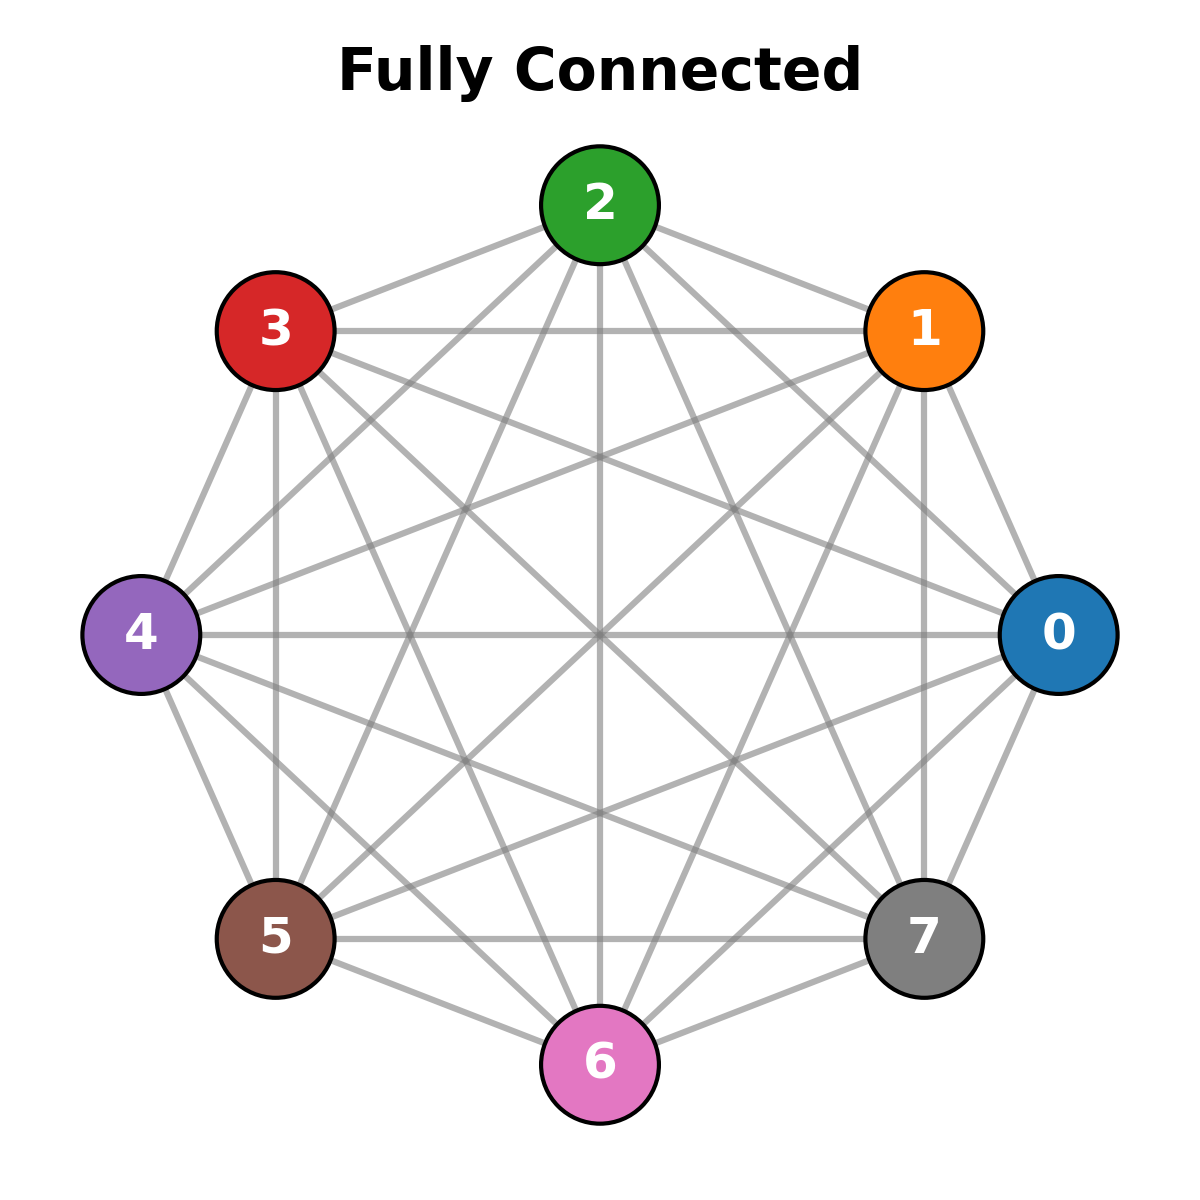
\includegraphics[width=0.3\textwidth]{figures/fc_colored.png}\\[0.5em]
    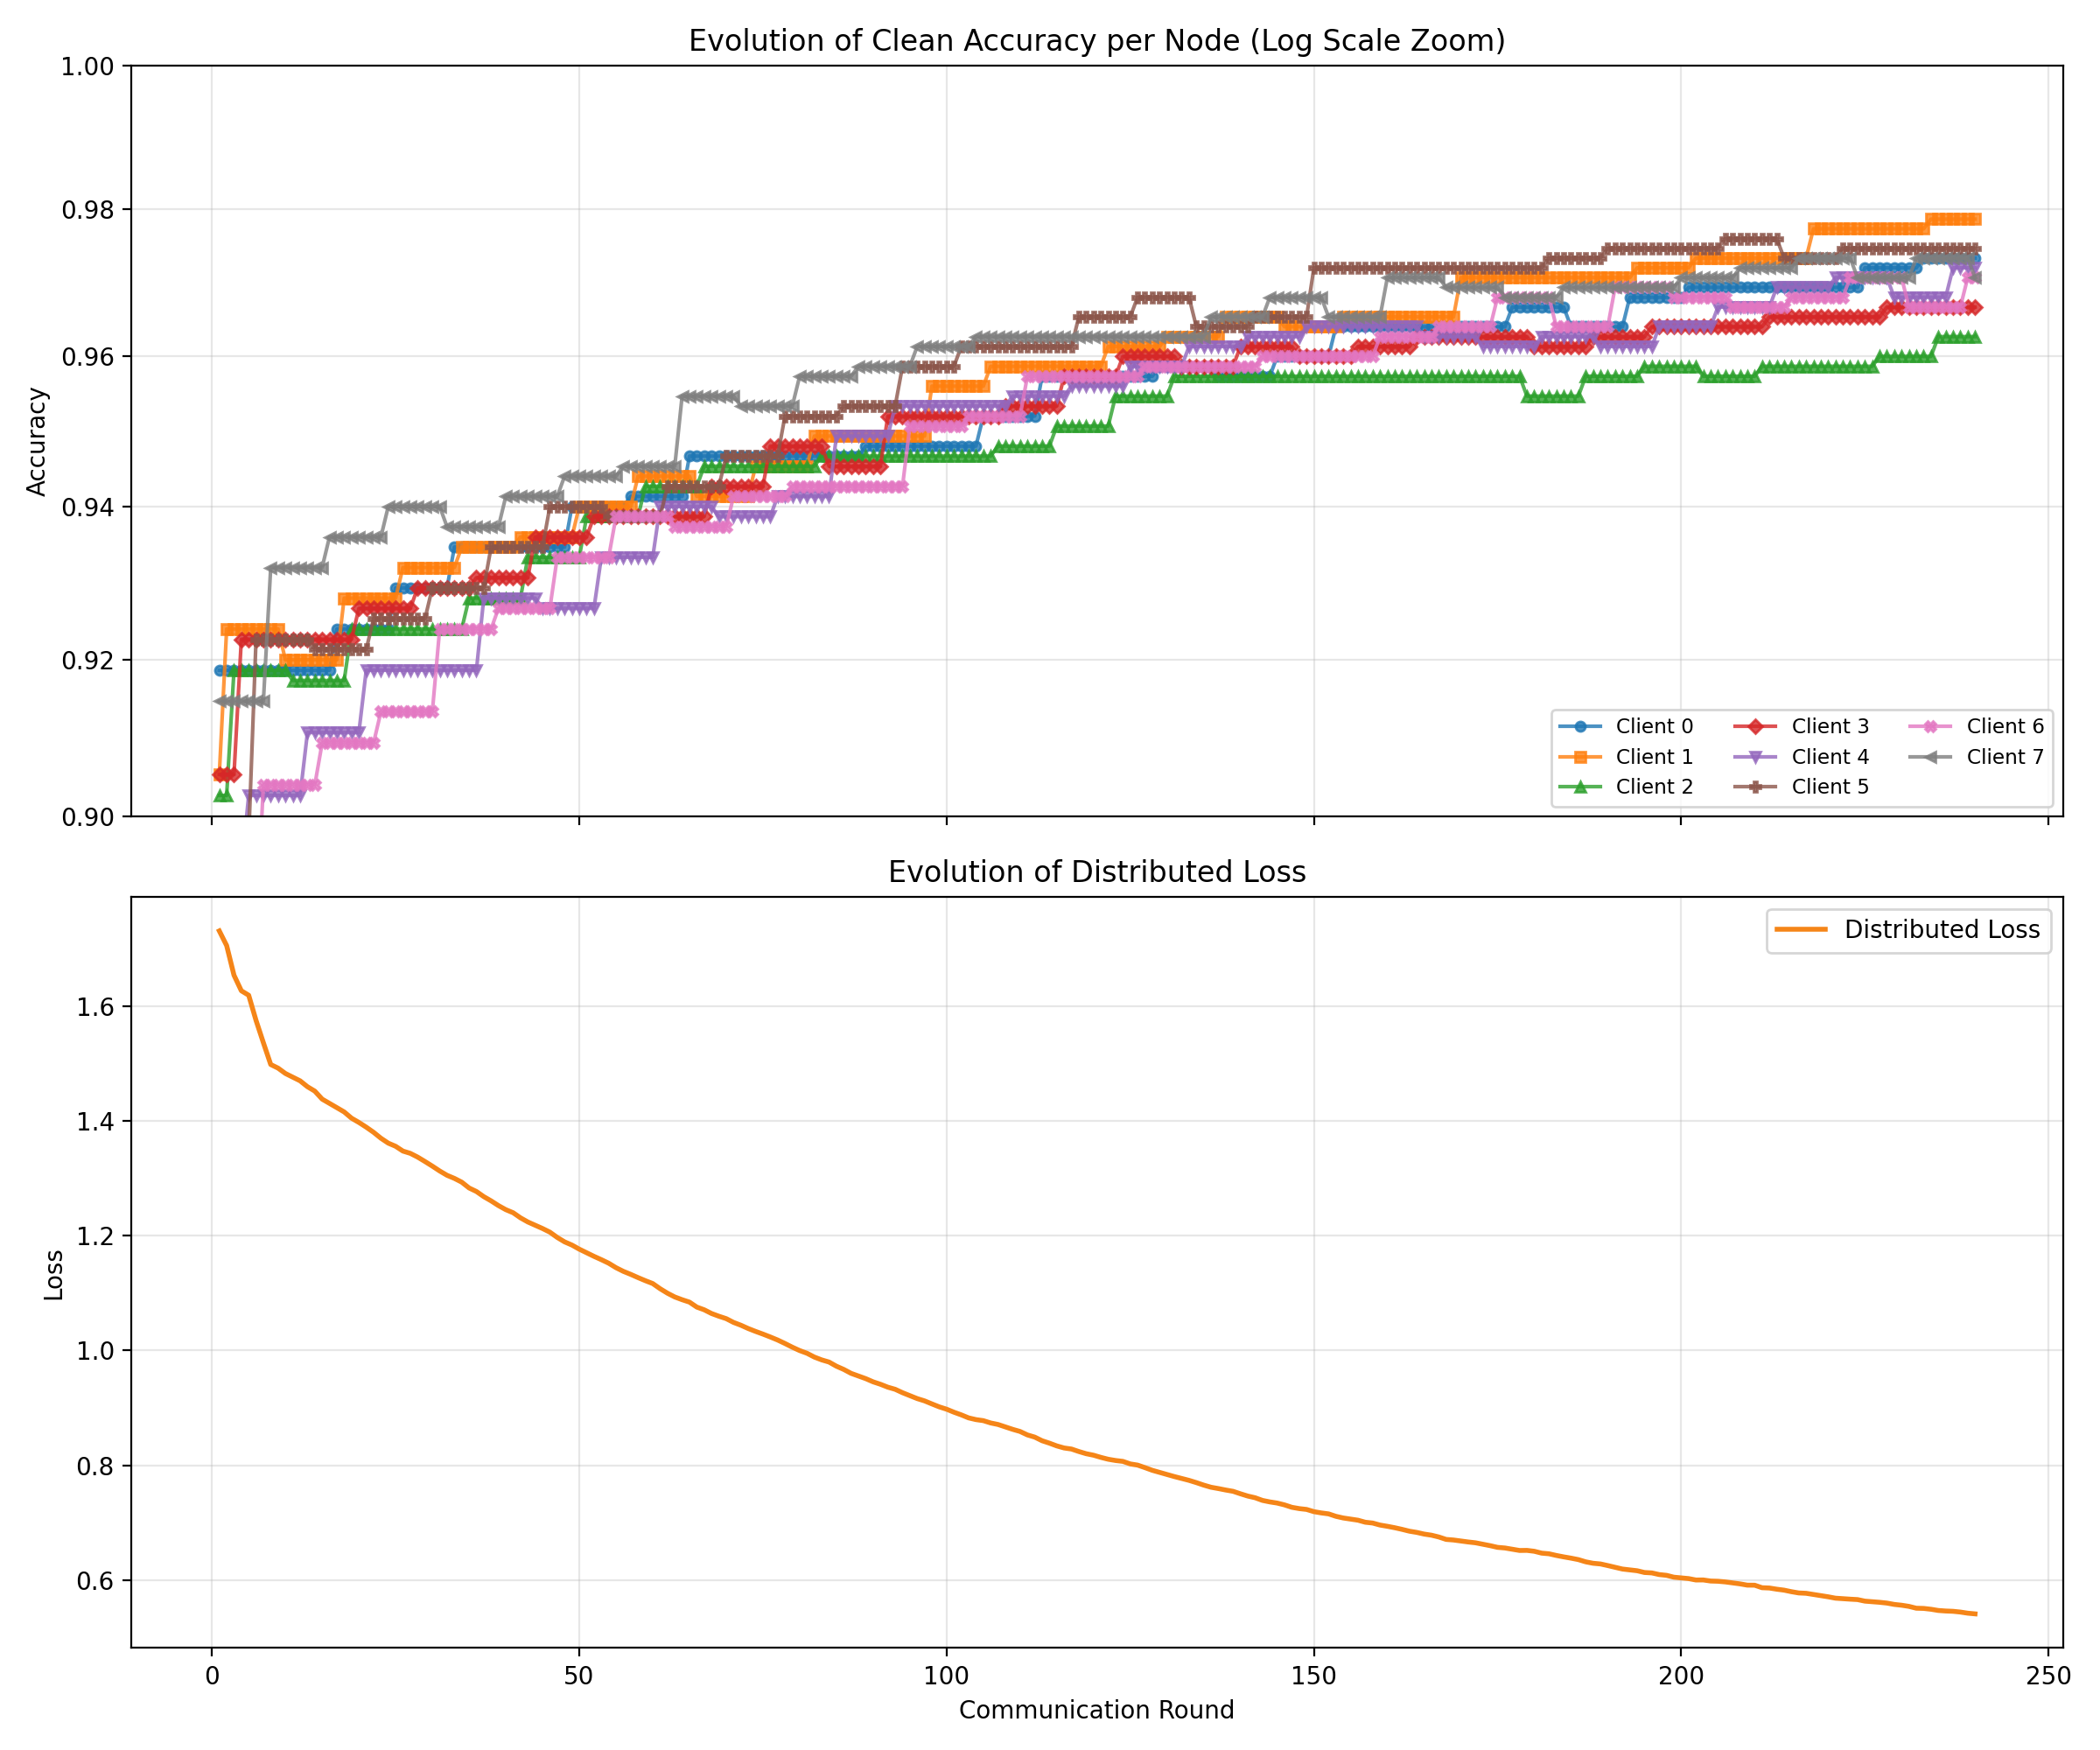
\includegraphics[width=1\textwidth]{figures/fc_clean.png}
    
    \caption{Baseline performance of the highly dense Fully Connected topology. The node colors in the graphs match the structural diagrams above.}
    \label{fig:app_baseline_row1}
\end{figure}

% --- ROW 2: Ring and Star ---
\begin{figure}[t]
    \centering
    % Top Image
    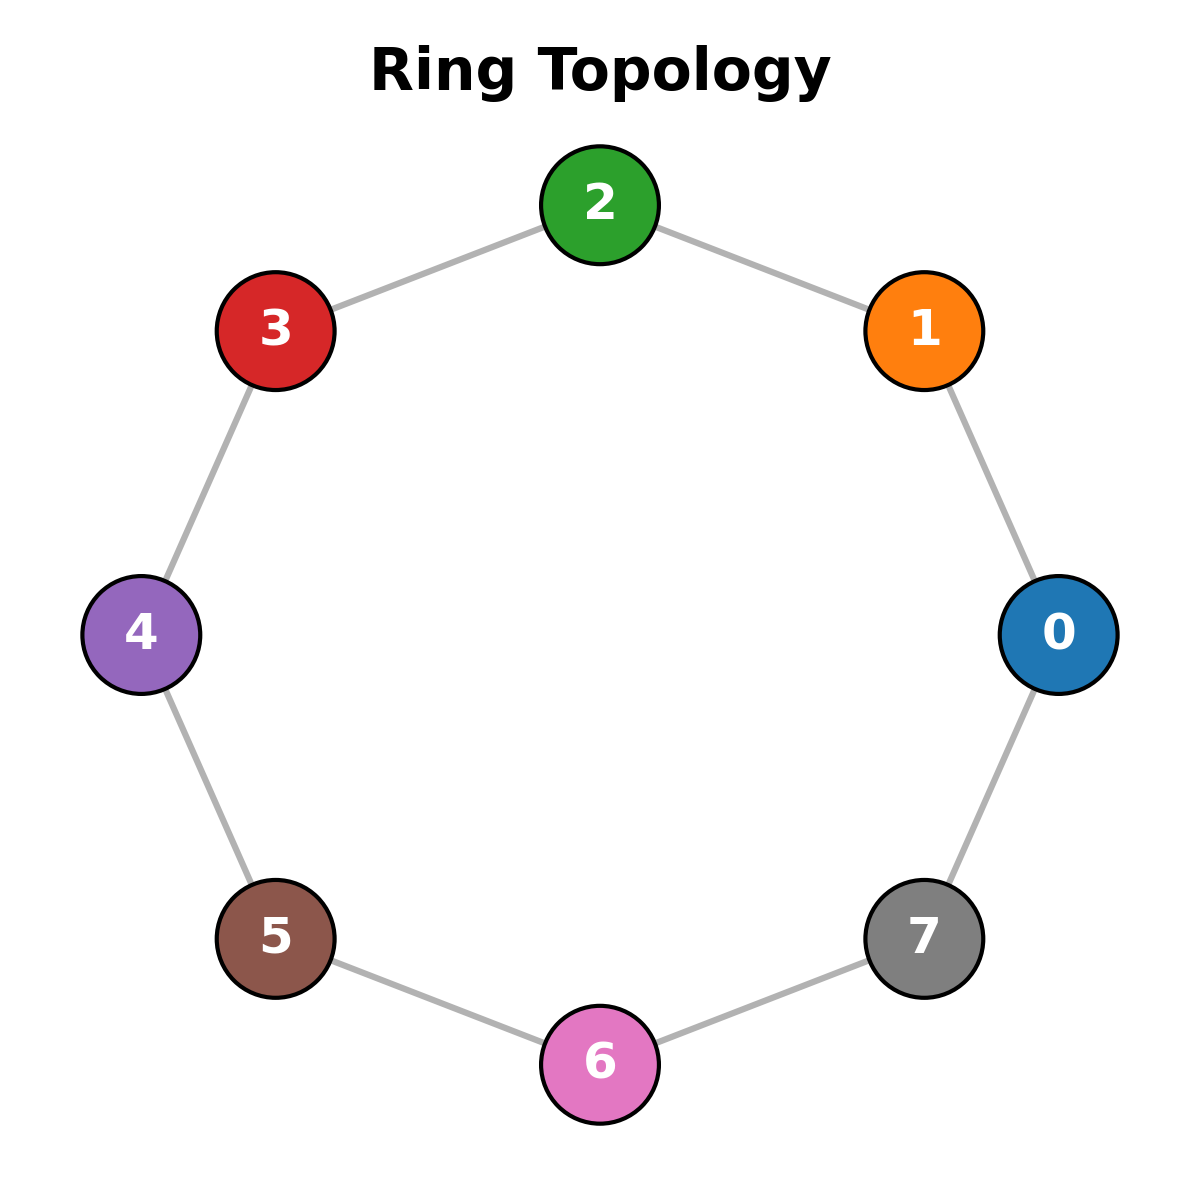
\includegraphics[width=0.3\textwidth]{figures/ring_colored.png}\\[0.5em]
    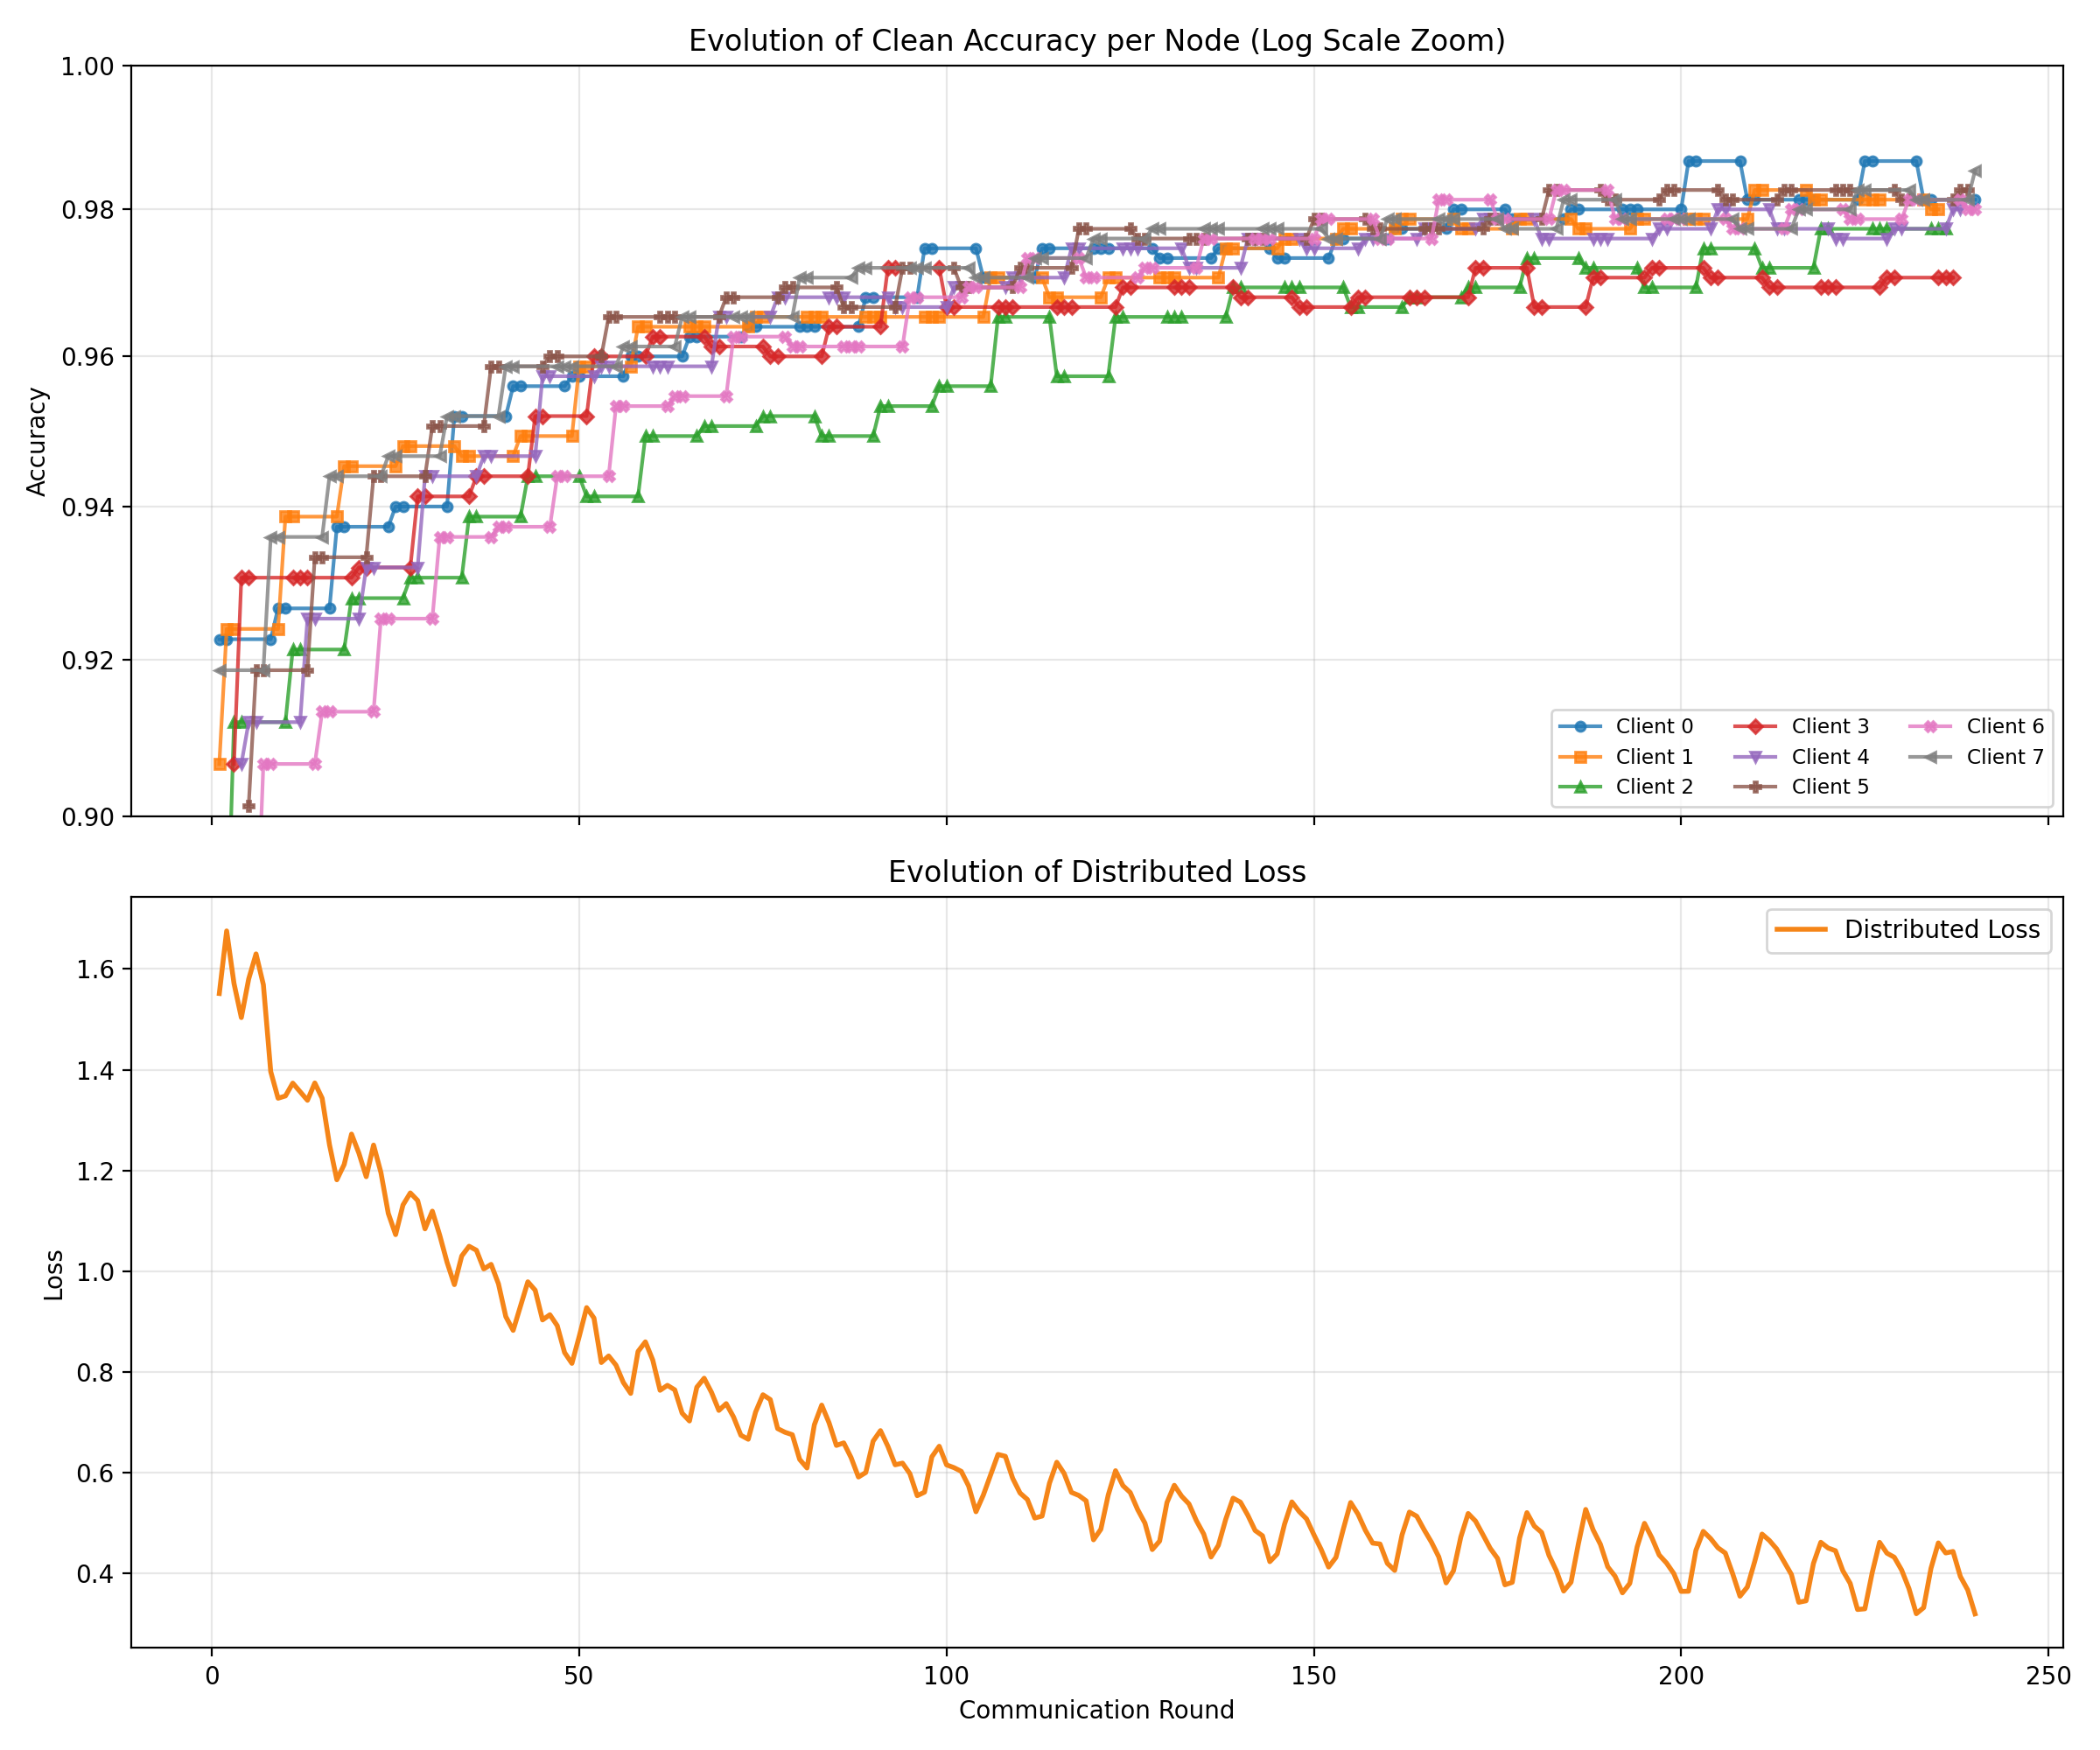
\includegraphics[width=1\textwidth]{figures/ring_clean.png}
    
    \vspace{0.8cm}
    
    % Bottom Image
    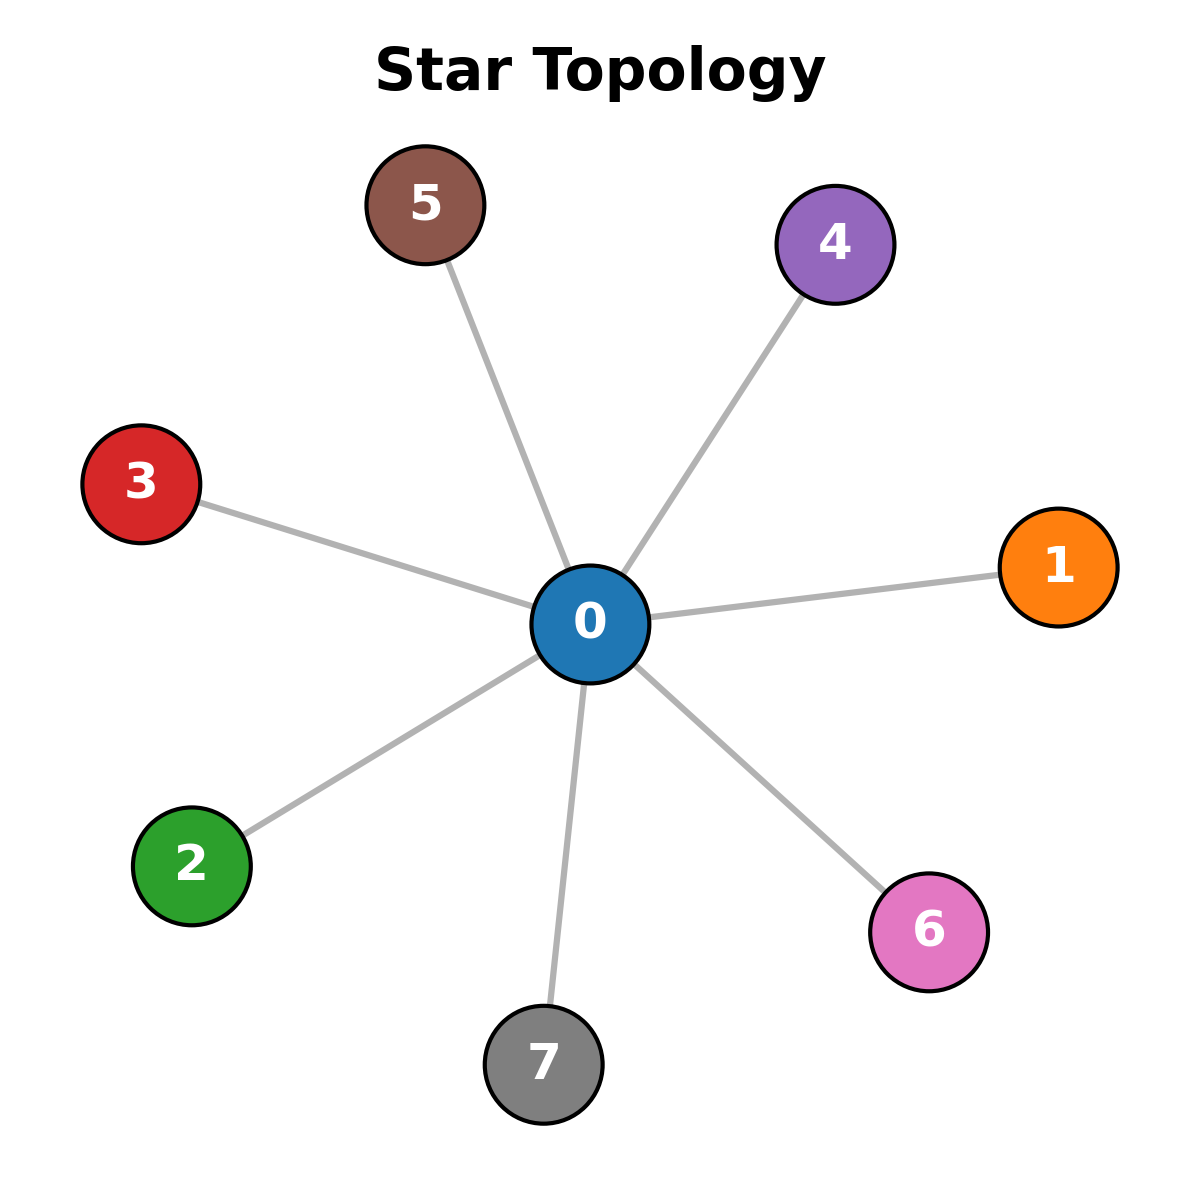
\includegraphics[width=0.3\textwidth]{figures/star_colored.png}\\[0.5em]
    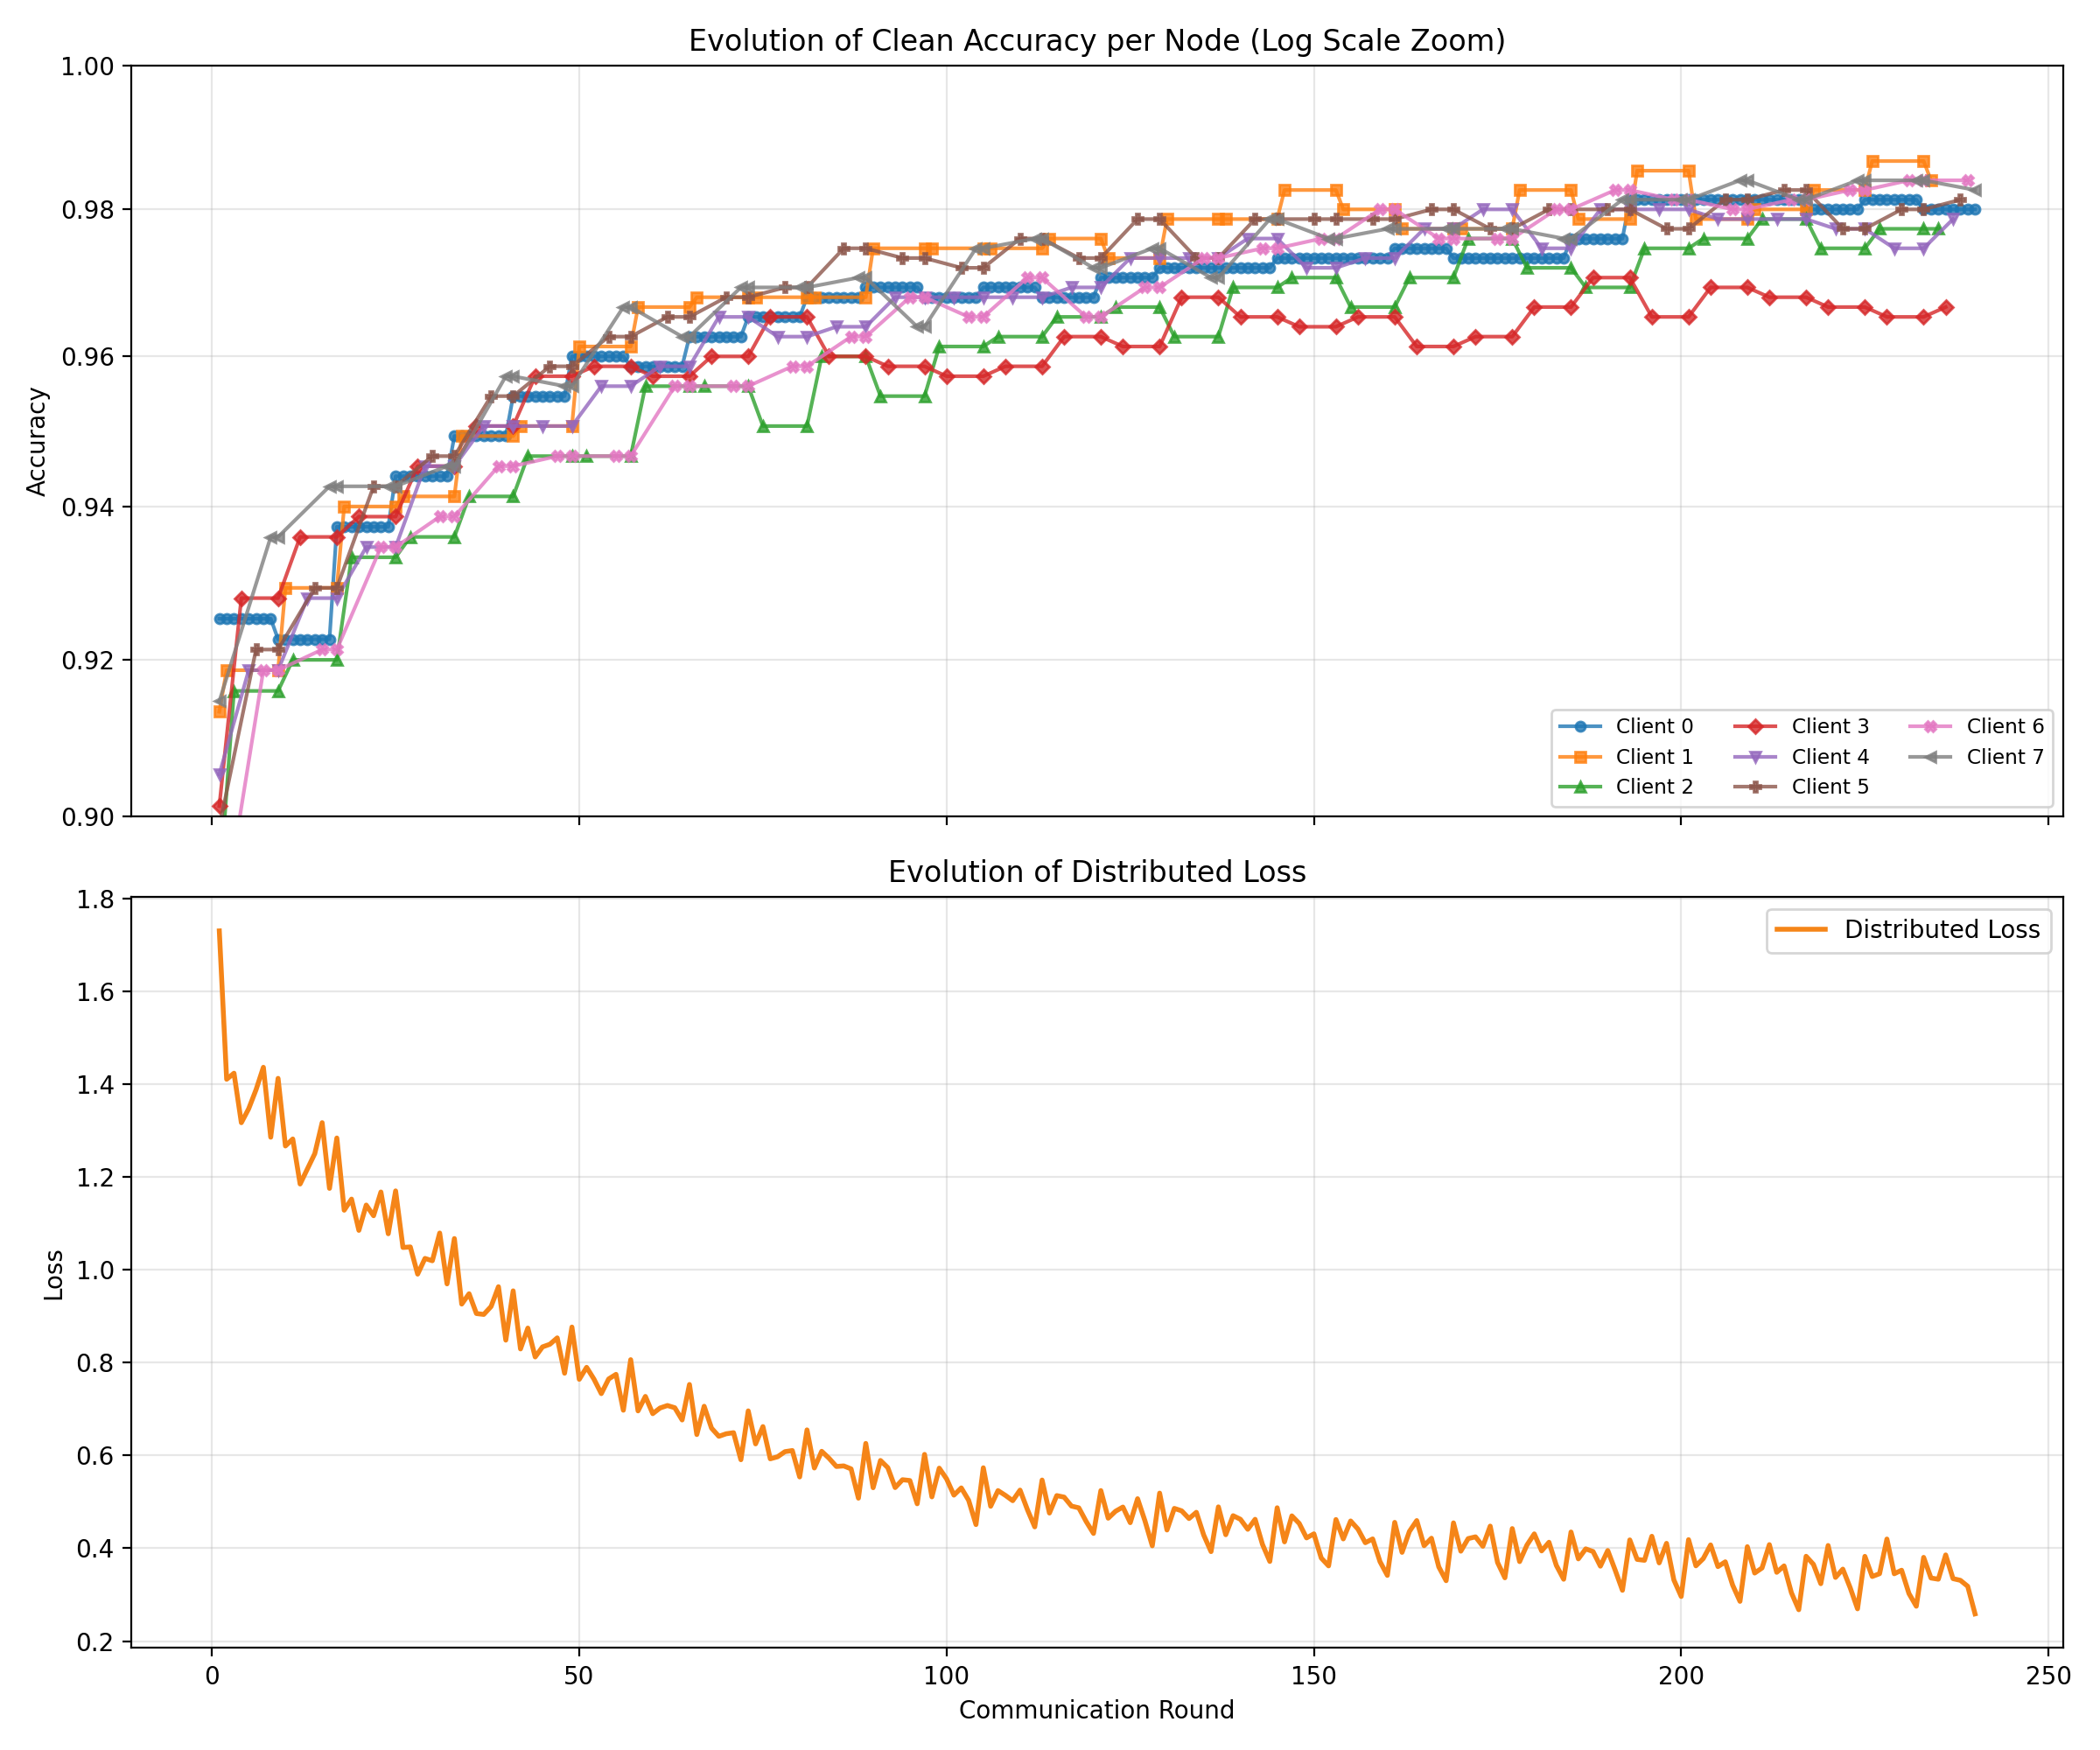
\includegraphics[width=1\textwidth]{figures/star_clean.png}
    
    \caption{Baseline performance comparison between the sparse Ring topology (top) and the centralized Star topology (bottom).}
    \label{fig:app_baseline_row2}
\end{figure}

% --- ROW 3: SBM ---
\begin{figure}[t]
    \centering
    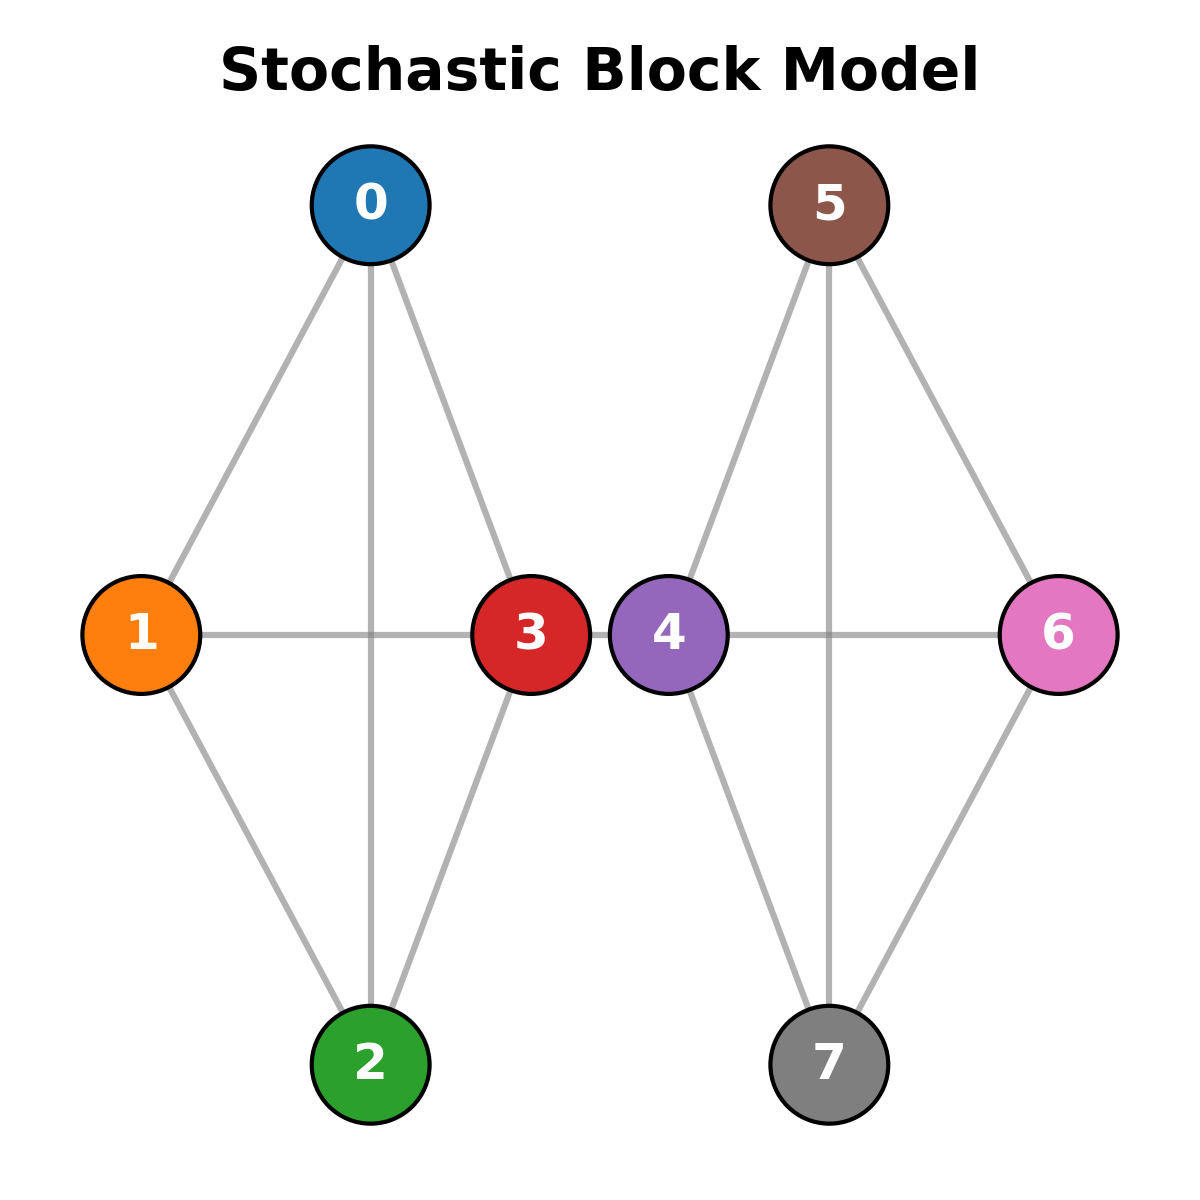
\includegraphics[width=0.3\textwidth]{figures/sbm_colored.png}\\[0.5em]
    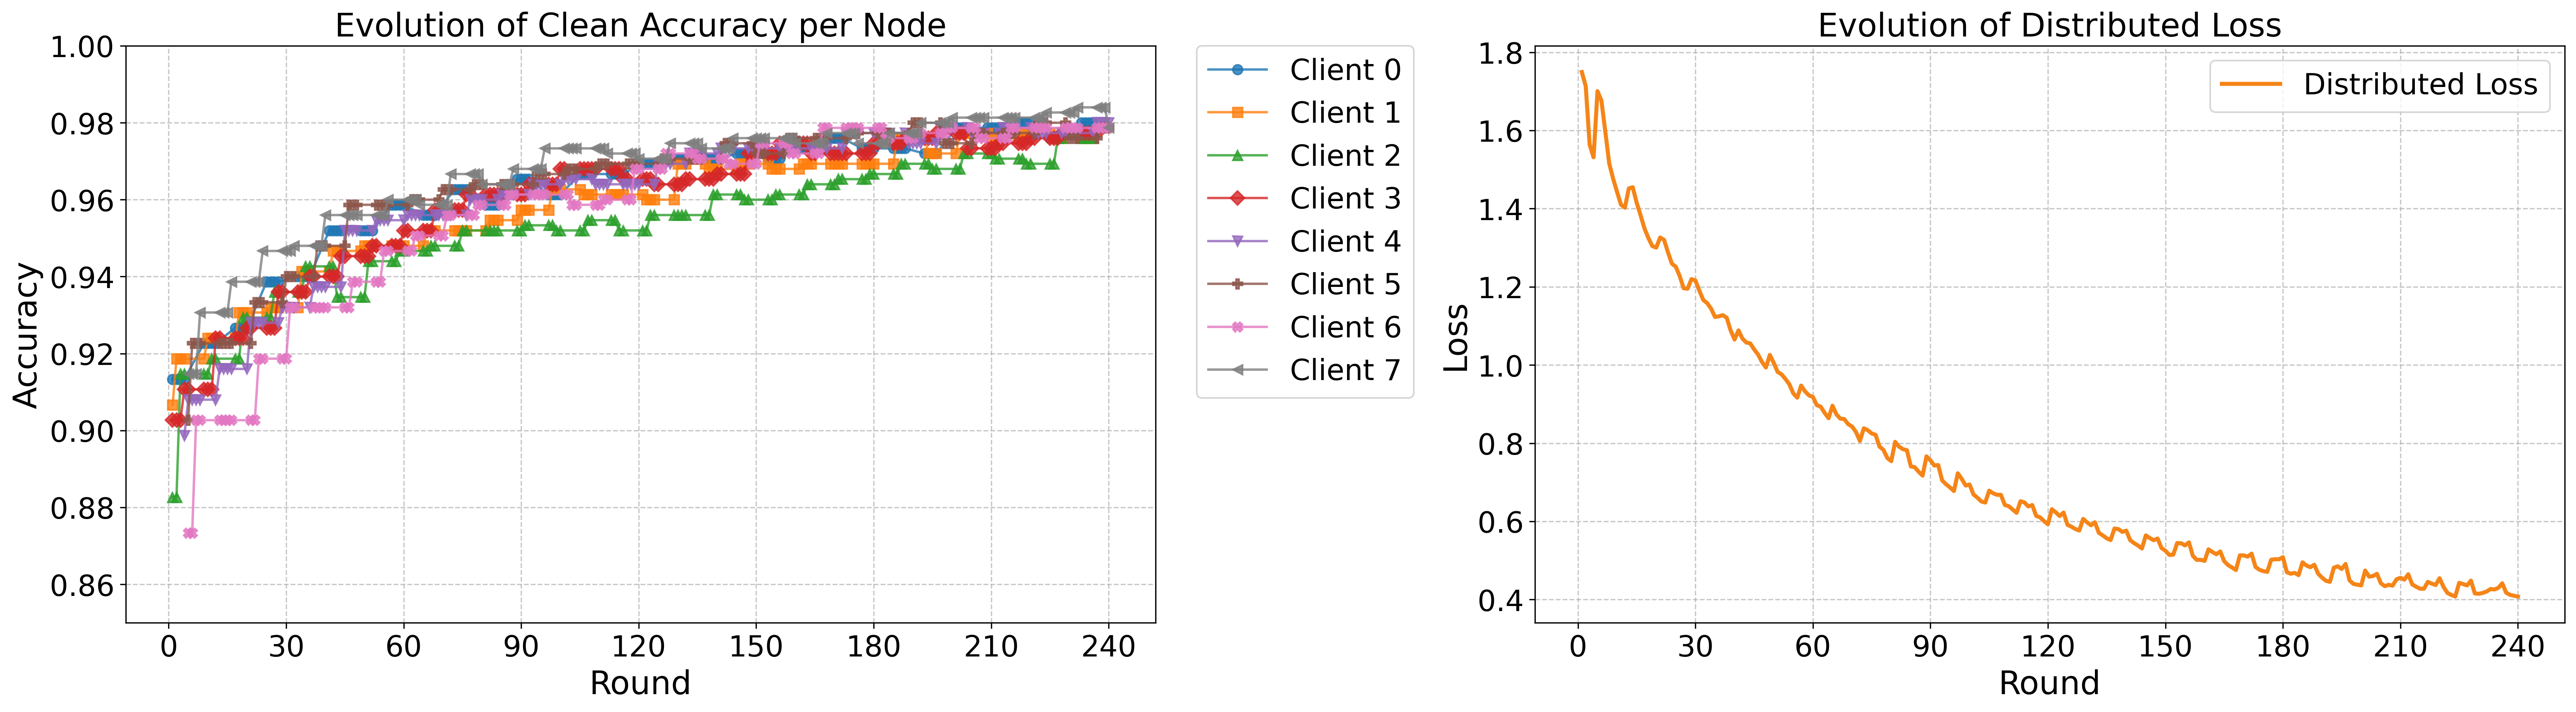
\includegraphics[width=1\textwidth]{figures/sbm_clean.png}
    \caption{Baseline performance for the Stochastic Block Model (SBM) topology, illustrating the natural convergence dynamics across two distinct communities.}
    \label{fig:app_baseline_row3}
\end{figure}

\clearpage
\section{Adversarial Evaluations}

The following figure (Figure \ref{fig:app_adv_row1}) represents the complete 240-round performance metrics for all nodes under a continuous backdoor attack in the Fully Connected topology. The attacker is positioned at Client 1 (Orange). The top figure illustrates the network topology, with node colors matching the individual client lines in the subsequent plots. This comprehensive visualization allows for a detailed assessment of how the adversarial payload propagates through a maximally dense network, highlighting both the rapid infection dynamics and the uniformity of convergence among honest nodes.

% --- ROW 1: FC and Ring ---
\begin{figure}[t]
    \centering
    % Top Image
    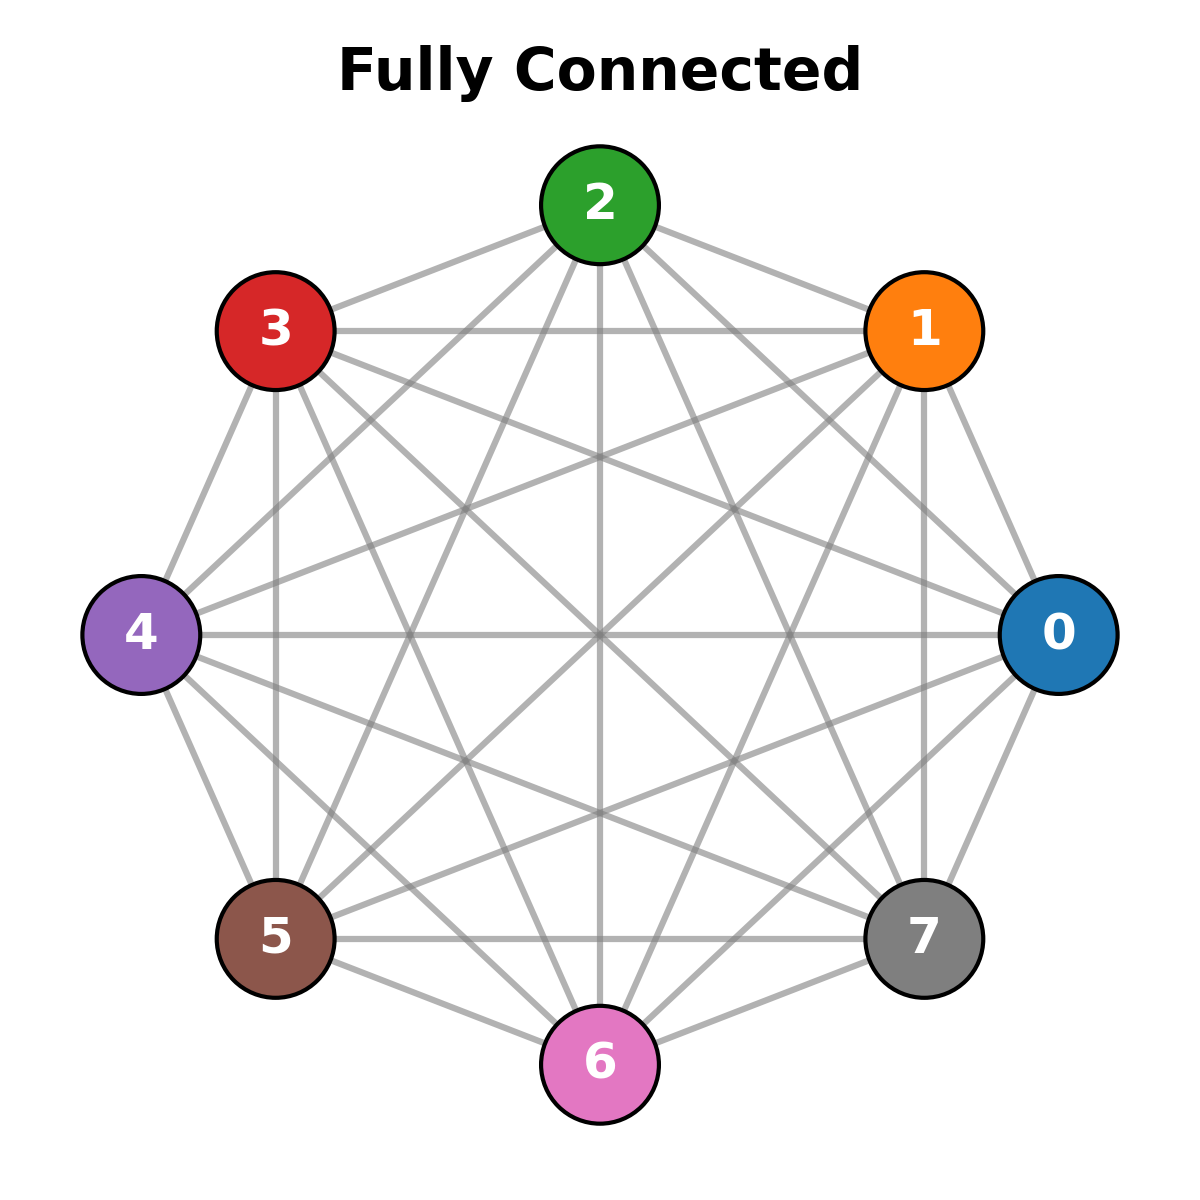
\includegraphics[width=0.3\textwidth]{figures/fc_colored.png}\\[0.5em]
    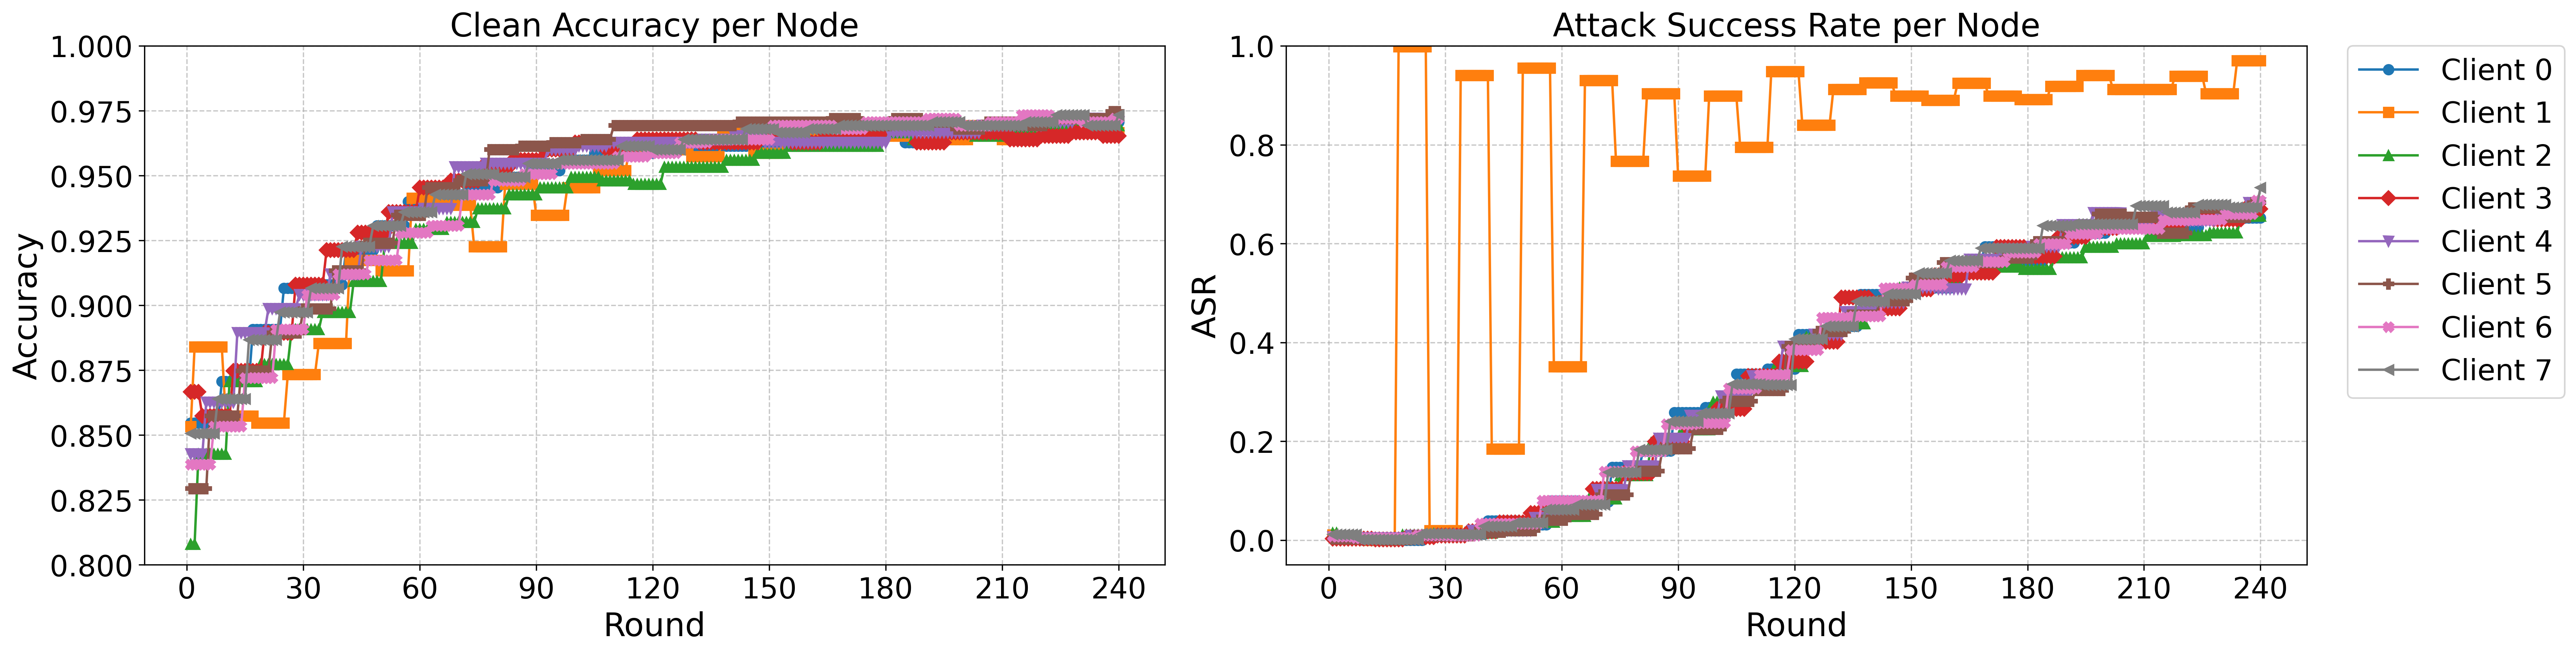
\includegraphics[width=1\textwidth]{figures/metrics_per_node_fc.png}
    
    \caption{Adversarial evaluation comparing a system-wide infection in the Fully Connected topology. The attacker is positioned at Client 1 (Orange).}
    \label{fig:app_adv_row1}
\end{figure}
